\documentclass[11pt,a4paper]{article}
\usepackage[margin=2.2cm]{geometry}
\usepackage{amsmath,amssymb}
\usepackage{booktabs}
\usepackage{graphicx}
\usepackage{float}
\usepackage{flafter}
\usepackage{xcolor}
\usepackage{microtype}
\usepackage{caption}
\usepackage{subcaption}
\usepackage{fancyhdr}
\usepackage[hidelinks]{hyperref}
\usepackage{enumitem}

\definecolor{accent}{HTML}{155E75}
\definecolor{soft}{HTML}{ECFEFF}
\hypersetup{colorlinks=true,linkcolor=accent,urlcolor=accent,citecolor=accent}
\captionsetup{font=small,labelfont=bf}
\setlist{nosep,leftmargin=1.5em}
\setlength{\parindent}{0pt}
\setlength{\parskip}{0.55em}
\pagestyle{fancy}
\setlength{\headheight}{14pt}
\fancyhf{}
\lhead{Signals and Systems Course Project}
\rhead{Anonymized portfolio edition}
\cfoot{\thepage}

\newcommand{\code}[1]{\texttt{#1}}
\newcommand{\dd}{\,\mathrm{d}}

\begin{document}

\begin{titlepage}
  \centering
  \vspace*{2.0cm}
  {\Large Signals and Systems\par}
  \vspace{0.6cm}
  {\color{accent}\rule{0.82\textwidth}{1.2pt}\par}
  \vspace{0.9cm}
  {\Huge\bfseries Audio-Signal Transformations and\\[0.25em]
  Stereo Vocal Reduction\par}
  \vspace{0.7cm}
  {\Large Course Project Report\par}
  \vfill
  \begin{minipage}{0.82\textwidth}
    \colorbox{soft}{\parbox{0.94\textwidth}{
      \textbf{Portfolio edition.} This report removes personal identifiers,
      separates reproducible evidence from subjective listening, and adds a
      controlled ground-truth experiment for the vocal-reduction methods.
    }}
  \end{minipage}
  \vfill
  {\large Author information withheld\par}
  \vspace{0.3cm}
  {\large October 2026\par}
\end{titlepage}

\begin{abstract}
This project applies core signals-and-systems concepts to digital audio. The
first part demonstrates time reversal and scaling, the discrete Fourier
transform (DFT), magnitude-only and phase-only reconstruction, and ideal
low-pass filtering. The second part studies stereo centre cancellation as a
simple vocal-reduction technique. In addition to the original $L-R$ baseline
and a low-frequency ``bass rescue'' variant, this edition introduces a
gain-and-delay compensated method for imperfectly centred vocals. A synthetic
benchmark with known vocal and accompaniment components shows the central
trade-off: under a two-sample, $0.82\times$ channel mismatch, compensation
improves vocal attenuation from $-10.69$ dB to $-26.54$ dB, while accompaniment
quality falls to $12.06$ dB SDR. The result is therefore an improvement for a
specific failure mode, not a universal vocal separator.
\end{abstract}

\tableofcontents
\newpage

\section{Objectives and implementation scope}

The course specification asks for two projects. Project~1 covers five
operations on a supplied audio signal: waveform display, time transformations,
frequency spectra, reconstruction from magnitude or phase, and ideal low-pass
filtering. Project~2 offers a choice of applications; this work implements the
voice-eliminator option and discusses both theory and practical improvement.

All processing is implemented in MATLAB. The public-facing repository excludes
the original songs, submission archives, student identifiers, and the course
handout. The controlled benchmark creates its own signals and therefore remains
fully reproducible without copyrighted audio.

\section{Project 1: time- and frequency-domain processing}

\subsection{Time transformations}

Let $f[n]$ be a sampled audio signal at sampling frequency $F_s$. Time reversal
is implemented by reversing the sample order. For a positive scale factor $a$,
the continuous-time relation $g(t)=f(at)$ is approximated on the original
sampling grid using linear interpolation:
\begin{equation}
  g[n] = f\!\left(a\frac{n}{F_s}\right).
\end{equation}
Values $a=3$ and $a=1/3$ produce compression and expansion respectively.
Figure~\ref{fig:time-transformations} shows the resulting duration changes.

\begin{figure}[htbp]
  \centering
  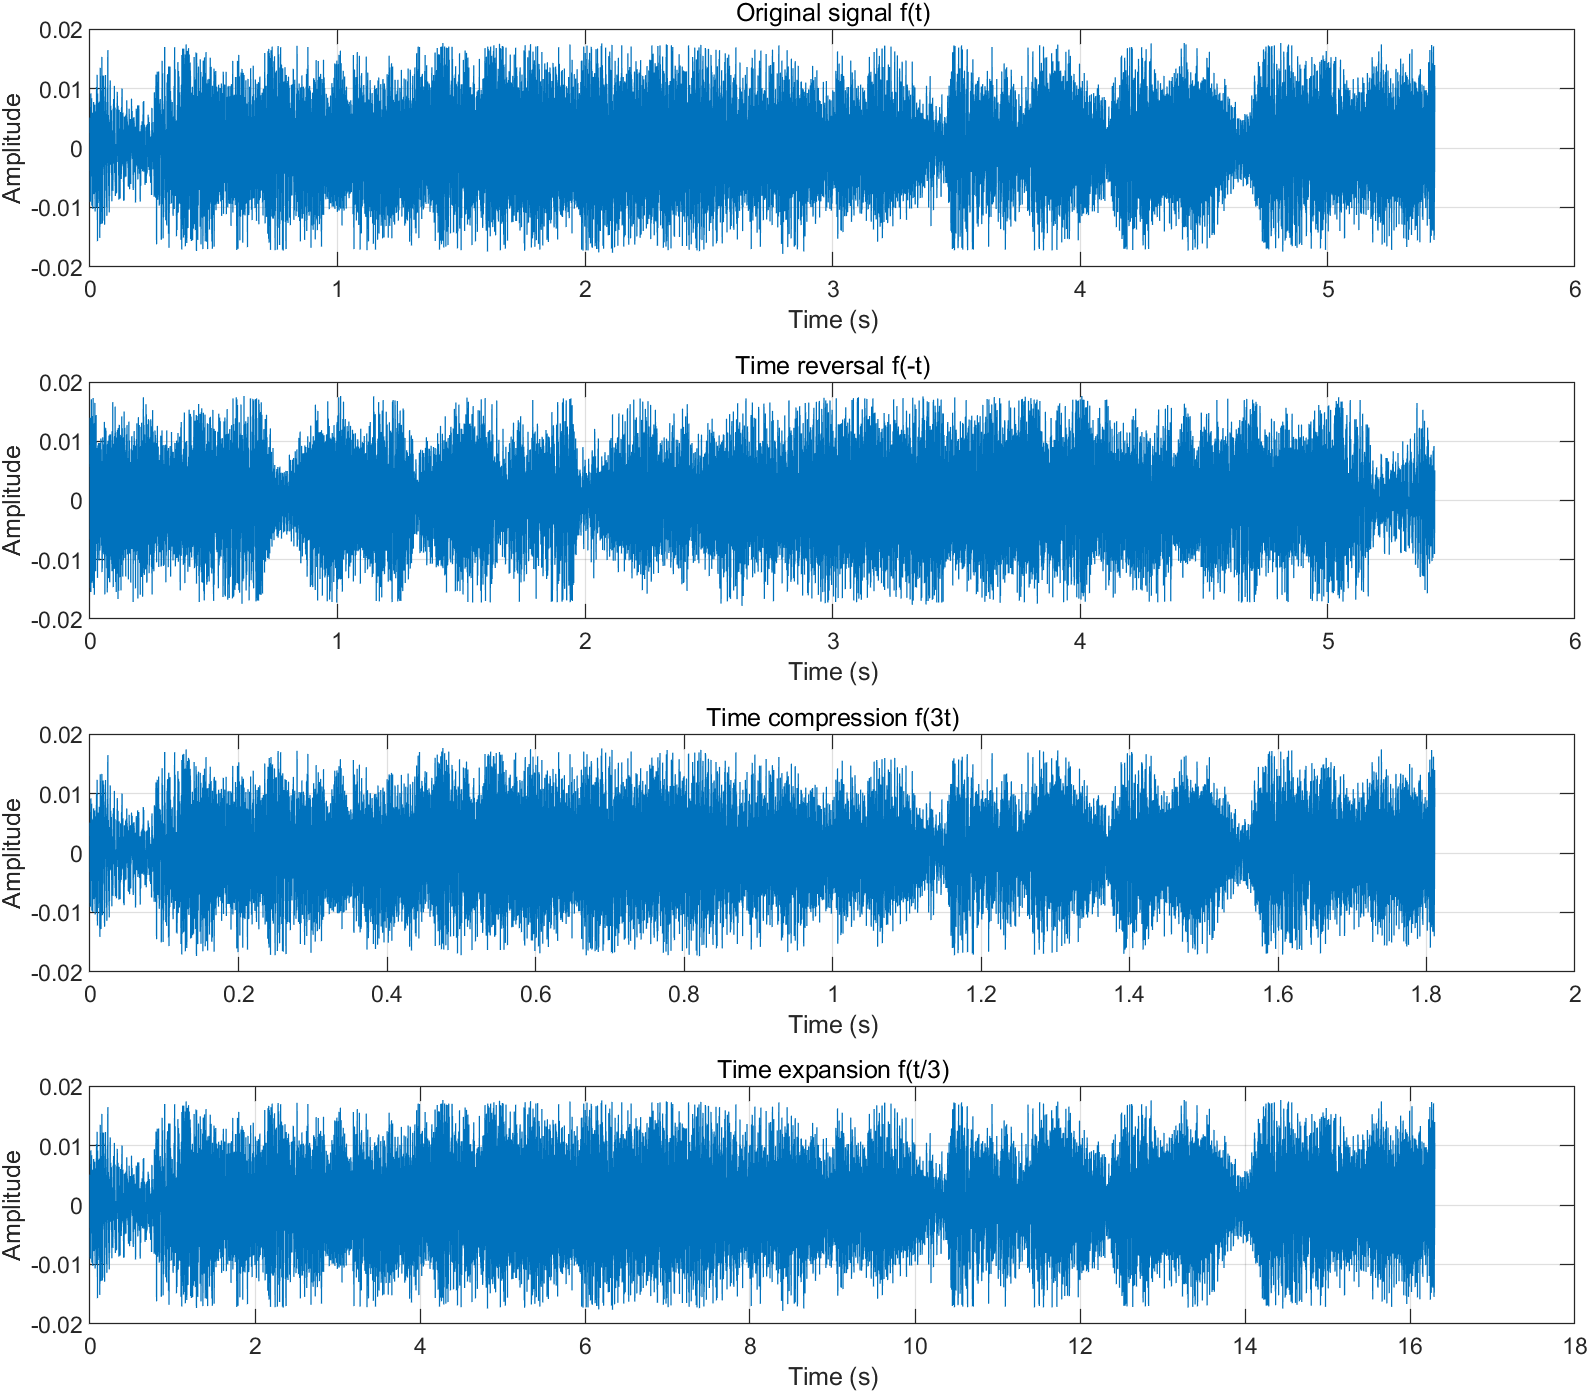
\includegraphics[width=0.92\textwidth]{../Project1/results/time_transformations.png}
  \caption{Original signal, time reversal, compression, and expansion. Each
  panel uses its own meaningful time span rather than forcing all plots onto
  the longest duration.}
  \label{fig:time-transformations}
\end{figure}

The interpolation is intentionally elementary. In a production resampler,
compression should include an anti-aliasing filter before samples are removed.
This limitation is retained and documented instead of being hidden by plotting.

\subsection{Discrete Fourier spectra}

For $N$ samples, the DFT is
\begin{equation}
  X[k] = \sum_{n=0}^{N-1} f[n]e^{-j2\pi kn/N}.
\end{equation}
The implementation uses exact DFT-bin frequencies, spaced by $F_s/N$, and
plots the normalized magnitude $|X[k]|/N$. This corrects the endpoint error
introduced by using \code{linspace(-Fs/2, Fs/2, N)} for a DFT axis.

\begin{figure}[htbp]
  \centering
  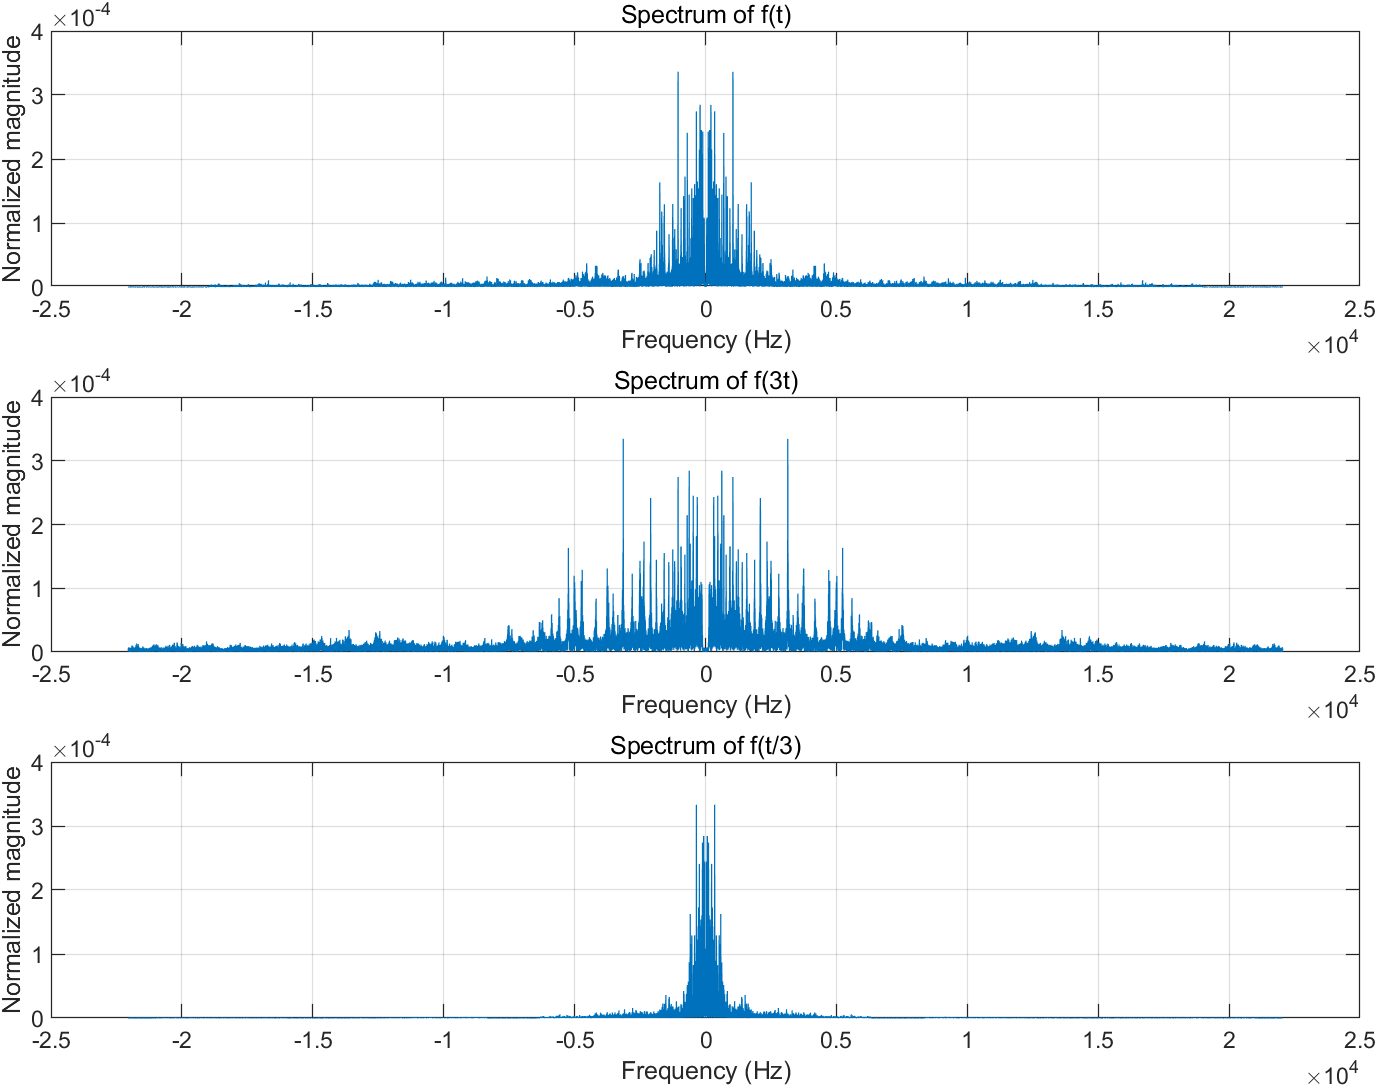
\includegraphics[width=0.92\textwidth]{../Project1/results/spectra.png}
  \caption{Normalized two-sided spectra for the original, compressed, and
  expanded signals. Time compression broadens spectral content; time expansion
  contracts it.}
  \label{fig:spectra}
\end{figure}

\subsection{Magnitude and phase reconstruction}

Writing $X[k]=|X[k]|e^{j\phi[k]}$, two deliberately incomplete inverse DFTs are
formed:
\begin{align}
  f_{\mathrm{mag}}[n] &= \operatorname{IDFT}\{|X[k]|\},\\
  f_{\mathrm{phase}}[n] &= \operatorname{IDFT}\{e^{j\phi[k]}\}.
\end{align}
The magnitude-only result preserves energy distribution but loses temporal
placement. The phase-only result has a very different amplitude scale yet can
retain recognizable timing structure. Figure~\ref{fig:phase} therefore avoids
claiming that either component alone reconstructs the original waveform.

\begin{figure}[htbp]
  \centering
  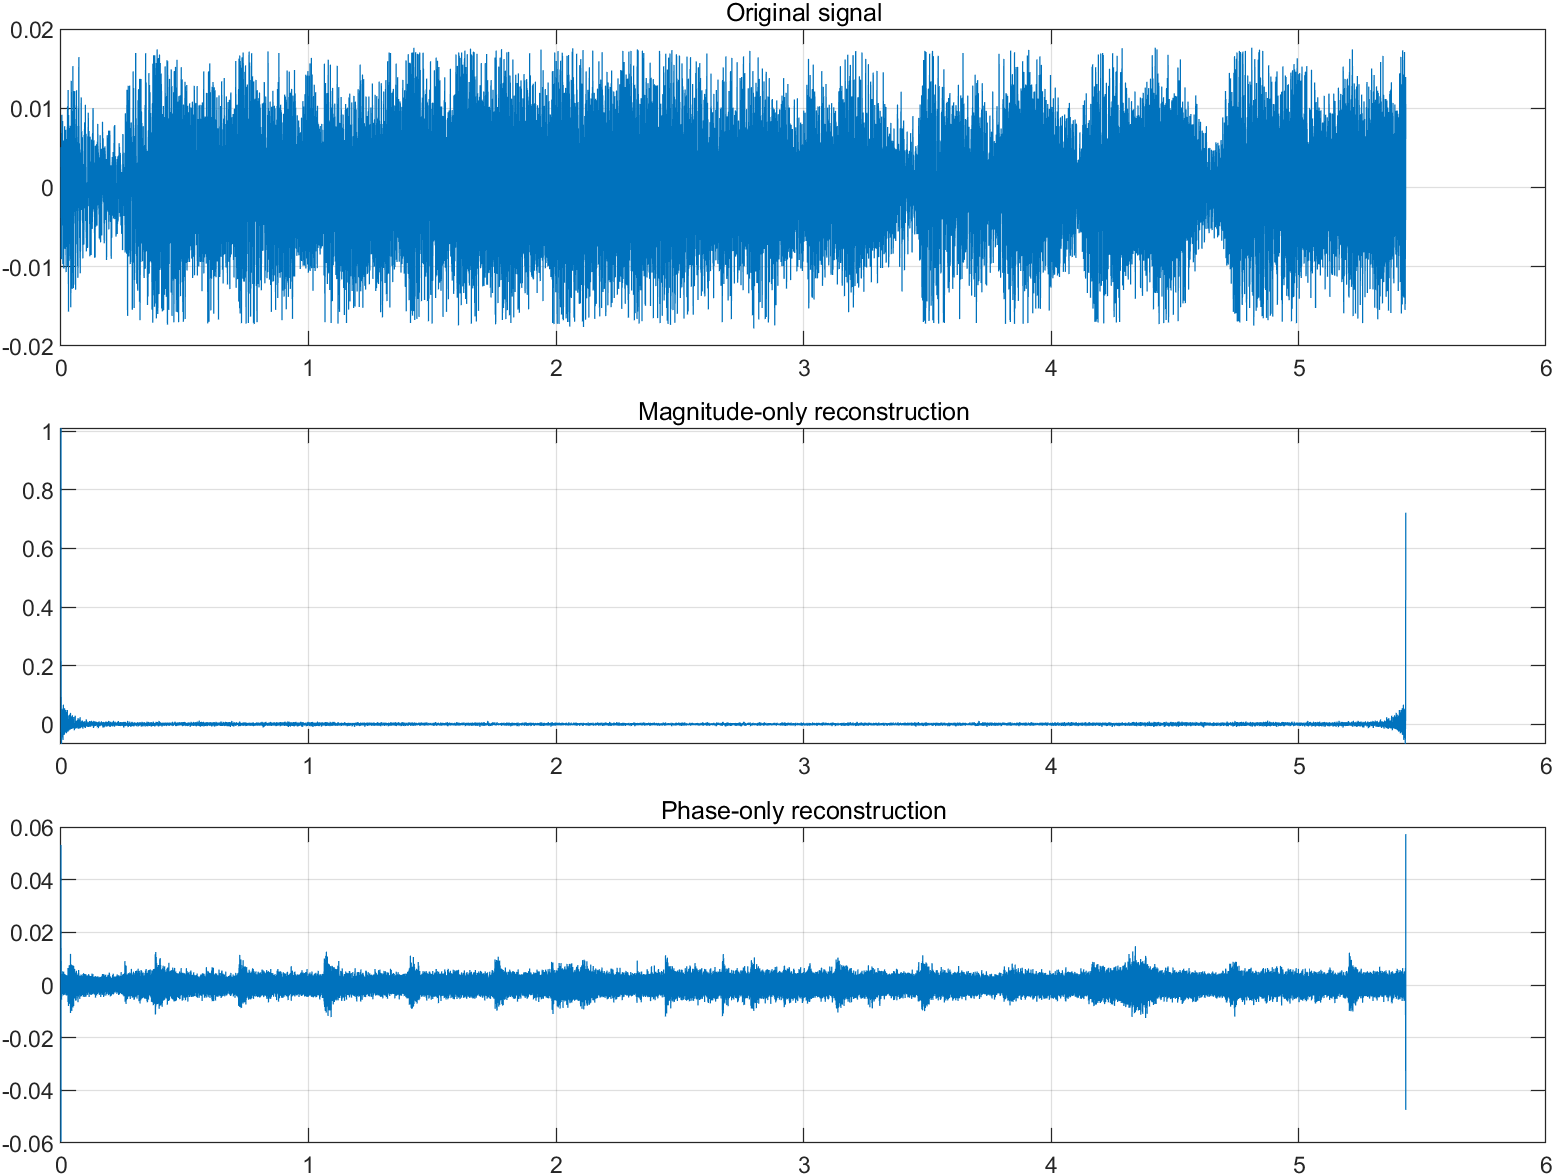
\includegraphics[width=0.92\textwidth]{../Project1/results/magnitude_phase_reconstruction.png}
  \caption{Original signal and inverse transforms using magnitude or phase
  information alone.}
  \label{fig:phase}
\end{figure}

\subsection{Ideal low-pass filtering}

The ideal frequency response is
\begin{equation}
  H(f)=\begin{cases}1,&|f|\leq f_c,\\0,&|f|>f_c,\end{cases}
  \qquad f_c=1000\ \mathrm{Hz},
\end{equation}
and the output is obtained from $y[n]=\operatorname{IDFT}\{X[k]H[k]\}$.

\begin{figure}[htbp]
  \centering
  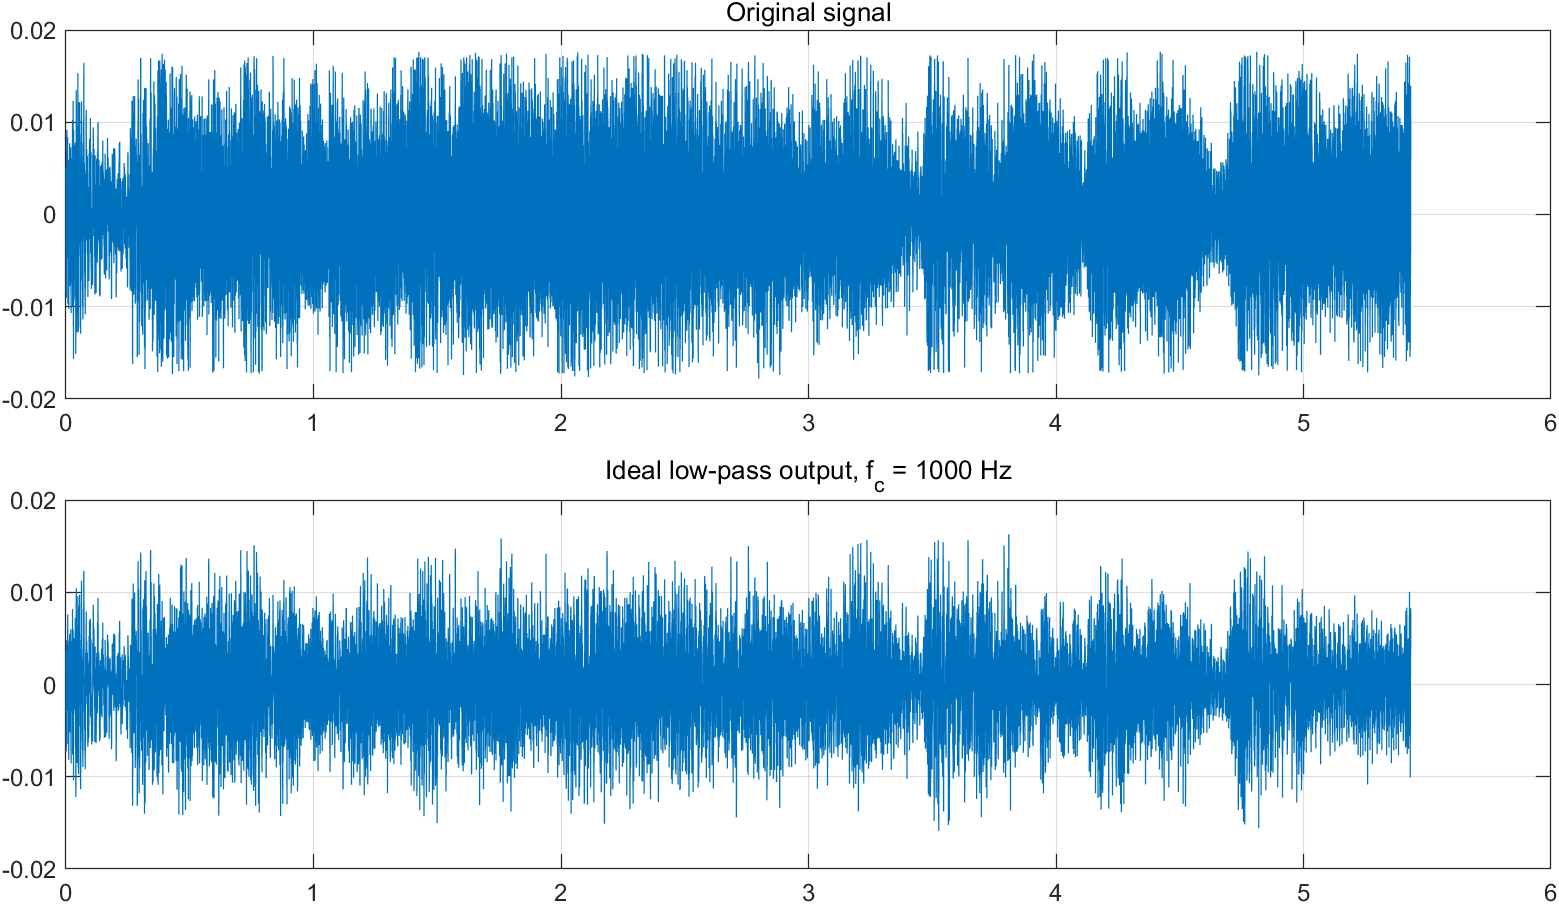
\includegraphics[width=0.92\textwidth]{../Project1/results/ideal_low_pass.png}
  \caption{Original signal and ideal low-pass output at $1$ kHz.}
  \label{fig:lpf}
\end{figure}

The implementation directly masks a finite-length DFT. Consequently it has a
brick-wall response, a long impulse response, circular boundary assumptions,
and possible ringing. Those are properties of the idealized exercise, not a
recommended real-time audio filter.

\section{Project 2: stereo vocal reduction}

\subsection{Stereo model and basic cancellation}

Assume a centre-panned vocal $v[n]$ and channel-dependent accompaniment
$a_L[n],a_R[n]$:
\begin{equation}
  L[n]=a_L[n]+v[n],\qquad R[n]=a_R[n]+v[n].
\end{equation}
Then
\begin{equation}
  y_{\mathrm{basic}}[n]=L[n]-R[n]=a_L[n]-a_R[n]
\end{equation}
cancels an exactly equal centre source. It also cancels every other equal
centre-panned element, including bass, kick, snare, and lead instruments.

\subsection{Legacy bass-rescue baseline}

The original extension added a low-frequency part of the mid channel:
\begin{equation}
  y_{\mathrm{bass}}[n]=L[n]-R[n]+0.30\,\operatorname{LPF}_{160\,\mathrm{Hz}}
  \left\{\frac{L[n]+R[n]}{2}\right\}.
\end{equation}
This can restore bass energy, but it is not unconditionally ``more advanced.''
Male vocal fundamentals can lie near or below the cutoff, so the method can
also reintroduce vocal content. It is kept as a documented legacy baseline.

\subsection{Gain-and-delay compensated cancellation}

Real mixes may place the nominal centre source in the two channels with a small
gain difference or sample delay. The improved method first isolates a broad
speech band ($120$--$6000$ Hz) for parameter estimation. It searches integer
delays $d\in[-8,8]$ and maximizes normalized correlation:
\begin{equation}
  \hat d=\arg\max_d
  \frac{\langle L_b,\,R_b(\cdot+d)\rangle}
  {\|L_b\|_2\,\|R_b(\cdot+d)\|_2}.
\end{equation}
After alignment, an energy-matching gain is estimated:
\begin{equation}
  \hat g=\sqrt{\frac{\|L_b\|_2^2}{\|R_b(\cdot+\hat d)\|_2^2}}.
\end{equation}
The gain is limited to $\pm6$ dB. Deviations smaller than $0.5$ dB are mapped
back to unity so that harmless stereo-energy differences do not spoil the exact
$L-R$ solution. Finally, a smooth frequency weight $W[k]$ blends the compensated
and basic outputs:
\begin{equation}
  Y[k]=(1-W[k])\,\mathcal{F}\{L-R\}
  +W[k],\mathcal{F}\{L-\hat gR(\cdot+\hat d)\}.
\end{equation}
The weight approaches one in the speech band and zero outside it. This limits
the scope of the compensation and avoids an abrupt rectangular band edge.

\section{Controlled experiment}

\subsection{Why a synthetic benchmark is necessary}

With a commercial stereo song, the isolated vocal and instrumental stems are
unknown. Waveform appearance, channel correlation, and listening impressions
cannot measure vocal attenuation objectively. The benchmark therefore creates
an eight-second stereo mixture from known components:
\begin{itemize}
  \item a harmonic, amplitude-modulated vocal-like centre source;
  \item different tonal and filtered-noise accompaniment in each channel;
  \item a shared $75$ Hz bass component;
  \item either ideal centring or a $0.82\times$ gain and two-sample delay in the
  right-channel vocal.
\end{itemize}

Every learned model is estimated from the mixture and then applied unchanged to
the known vocal and accompaniment components. Three metrics are reported:
vocal leakage attenuation relative to the input vocal; scale-invariant
accompaniment signal-to-distortion ratio (SDR); and the accompaniment-to-vocal
energy ratio at the output. Values at $\pm80$ dB indicate the numerical display
floor or ceiling rather than infinite physical performance.

\begin{table}[H]
  \centering
  \caption{Controlled benchmark results. Lower vocal attenuation is better;
  higher SDR and output ratio are better.}
  \label{tab:benchmark}
  \small
  \begin{tabular}{llrrr}
    \toprule
    Scenario & Method & Vocal attn. (dB) & Acc. SDR (dB) & Output ratio (dB)\\
    \midrule
    Ideal centre & $L-R$ & $-80.00$ & $80.00$ & $80.00$\\
    Ideal centre & Bass rescue & $-61.50$ & $18.44$ & $60.26$\\
    Ideal centre & Adaptive & $-80.00$ & $80.00$ & $80.00$\\
    Gain + delay mismatch & $L-R$ & $-10.69$ & $80.00$ & $10.27$\\
    Gain + delay mismatch & Bass rescue & $-10.69$ & $18.44$ & $10.32$\\
    Gain + delay mismatch & Adaptive & $-26.54$ & $12.06$ & $26.80$\\
    \bottomrule
  \end{tabular}
\end{table}

\begin{figure}[htbp]
  \centering
  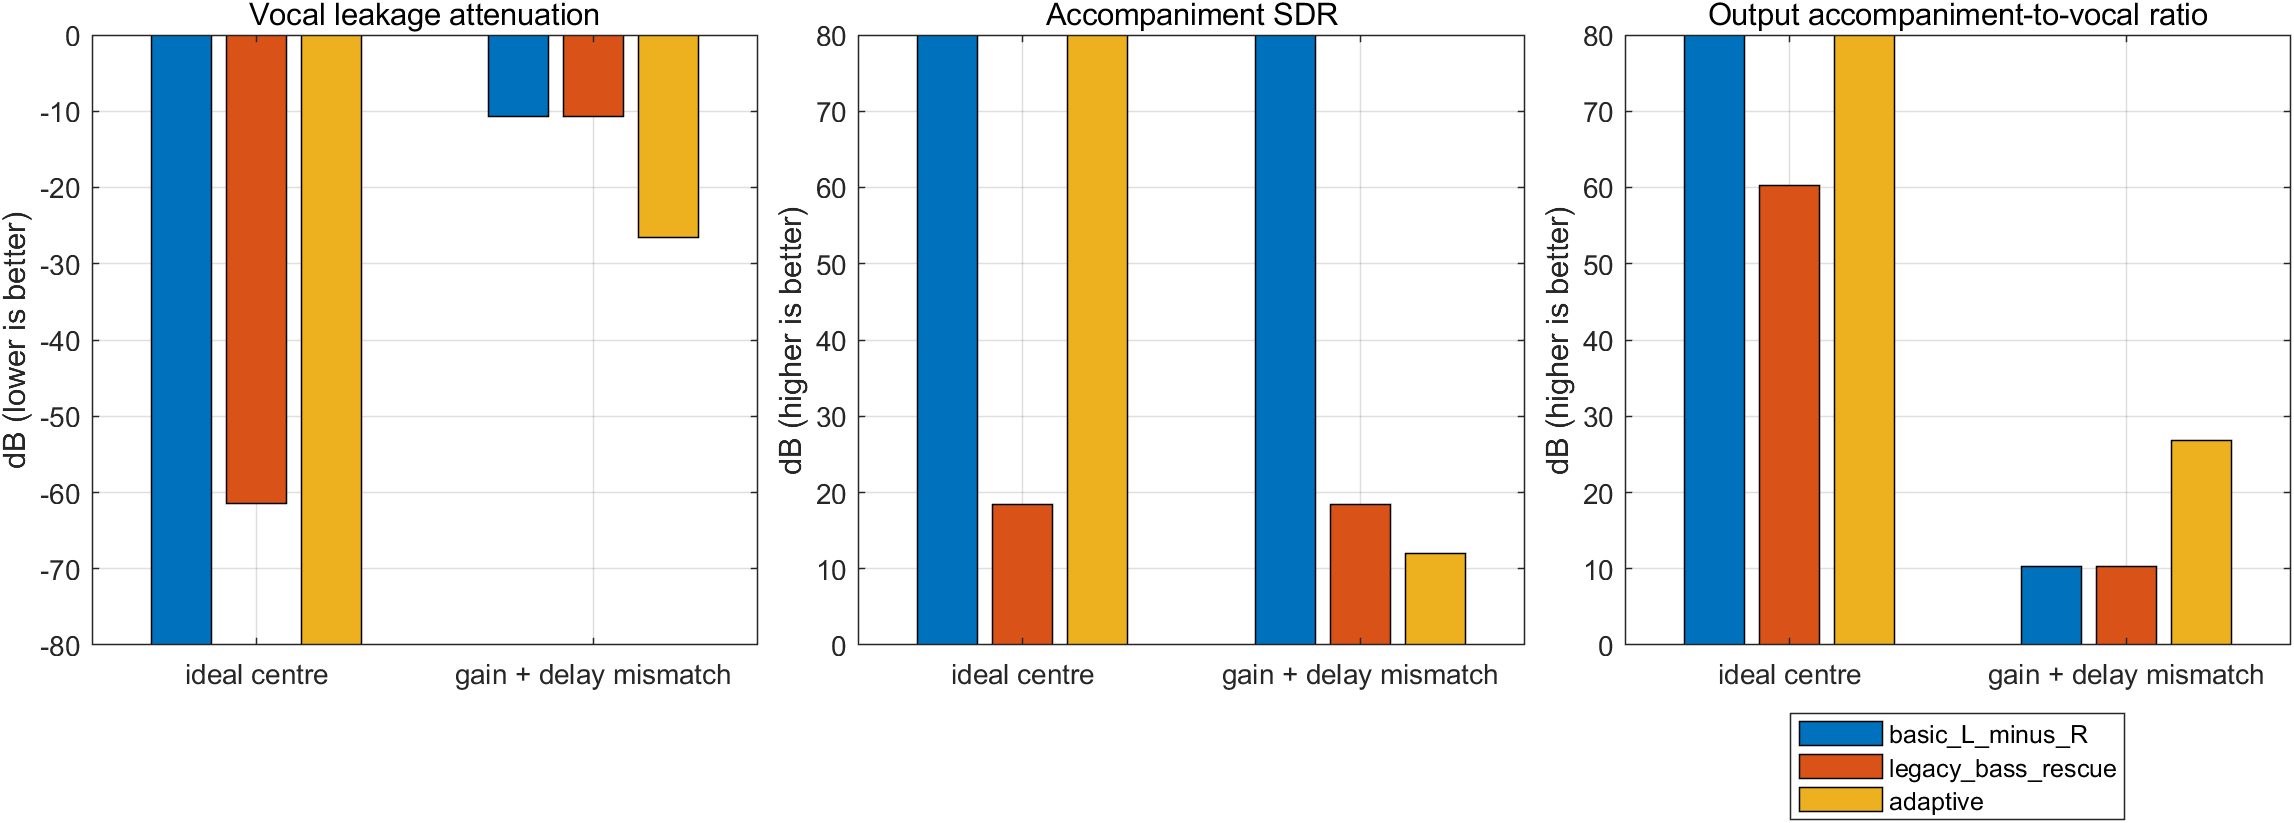
\includegraphics[width=\textwidth]{../Project2/experiments/results/benchmark_summary.png}
  \caption{Benchmark summary. The compensated method substantially reduces
  vocal leakage under channel mismatch, but it also changes the accompaniment.}
  \label{fig:benchmark}
\end{figure}

Under ideal centring, the simplest method is already optimal. Under mismatch,
the adaptive method gains $15.85$ dB of vocal attenuation and $16.54$ dB in the
output accompaniment-to-vocal ratio relative to $L-R$. Its $12.06$ dB
accompaniment SDR quantifies the cost. The result supports a conditional claim:
gain-and-delay compensation is useful when the centre-source assumption is
slightly violated, but it should not be enabled blindly.

\section{Real-audio diagnostics}

Two local stereo excerpts were processed for listening tests, but are excluded
from version control. Because isolated stems are unavailable, Table~\ref{tab:real}
reports only descriptive stereo statistics. They are not labelled as vocal
removal scores.

\begin{table}[H]
  \centering
  \caption{Descriptive statistics for local test excerpts.}
  \label{tab:real}
  \begin{tabular}{lrrrr}
    \toprule
    Case & $F_s$ (Hz) & Duration (s) & L/R correlation & Mid/side energy (dB)\\
    \midrule
    A & 44100 & 35.016 & 0.906 & 13.065\\
    B & 44100 & 23.057 & 0.705 & 7.618\\
    \bottomrule
  \end{tabular}
\end{table}

Case~A has stronger centre coherence and is consequently a more favourable
candidate for centre cancellation. Case~B contains more stereo-side energy, so
subtraction is less likely to isolate ``instrumental only'' content. Listening
tests remain useful for detecting musical artifacts, but they do not replace
the controlled metrics.

\section{Limitations and reproducibility}

\begin{itemize}
  \item Centre cancellation cannot distinguish vocals from other centred
  sources. Modern stem-separation systems solve a different, harder problem.
  \item A single global delay and gain cannot model time-varying reverberation,
  chorus effects, nonlinear processing, or frequency-dependent panning.
  \item The synthetic benchmark is deliberately controlled and does not span
  the full diversity of commercial mixes.
  \item Project~1 time compression uses interpolation without an anti-aliasing
  prefilter, and its ideal DFT filter has circular-boundary artifacts.
  \item Real-song outputs are normalized with one common safety factor per song,
  rather than separately, so relative levels remain comparable.
\end{itemize}

The repository scripts use paths relative to each MATLAB file, create their own
output directories, and generate figures non-interactively. The benchmark uses
a fixed random seed. Source audio and generated WAV files are ignored by Git;
the metrics CSV and figures are tracked.

\section{Conclusion}

The project now does more than demonstrate textbook operators. It shows where
the assumptions behind centre cancellation succeed, where the original
bass-rescue idea fails, and how a narrowly targeted correction changes both
vocal leakage and accompaniment fidelity. The strongest portfolio value lies in
this evidence-driven comparison: a simple baseline, a motivated improvement,
an objective benchmark, and an explicit account of limitations.

\begin{thebibliography}{9}
\bibitem{oppenheim}
A. V. Oppenheim and R. W. Schafer,
\textit{Discrete-Time Signal Processing}, 3rd ed., Pearson, 2010.

\bibitem{smith}
J. O. Smith III,
\textit{Spectral Audio Signal Processing}, W3K Publishing, 2011.

\bibitem{specification}
Signals and Systems course project specification, internal course handout, 2026.
\end{thebibliography}

\end{document}
